\chapter{Thermodynamik}
\section{Grundbegriffe der Thermodynamik}
\textbf{Energie E}\\
= Fähigkeit eines Systems Arbeit zu verrichten
\begin{itemize}
	\item kinet. E = $\frac{1}{2}*m*v^2$
	\item elektr. E = $U/d$
	\item pot. E = $m*g*h$
	\item Wärmeenergie = $m*c_p+\Delta T$ , wenn $p=const.$
	\item Photonenenergie = $h*f$
\end{itemize}

\textbf{Arbeit W}
\begin{itemize}
	\item mech. Arbeit = $F*s$
	\item elektr. Arbeit = $P*t=I^2*R*t$
	\item Volumenarbeit = $-p*\text{d}V$
\end{itemize}

\textbf{Leistung P} = $\frac{W}{t}$\\ \\

\textbf{\underline{Arten von Systemen:}}
\begin{itemize}
	\item \textbf{offenes System}: Energie und Stoff
	\item  \textbf{geschlossenes System}: Energie
	\item  \textbf{abgeschlossenes System}: nichts ("`adiabat"') 
\end{itemize}

\section{Ideales Gasgesetz}
\textbf{Satz von Avogadro}: \\
$V=\text{Konstante}*n$ für $T,p = const.$\\

\textbf{Gesetz von Gay-Lussac}: \\
$V=\text{Konstante}*T$ für $n,p = const.$\\

\textbf{Boyle-Marriot'sche Gasgesetz}: \\
$p*V=const.$ für $n,T = const.$\\

\textbf{Ideales Gasgesetz}: \\
$\frac{p*V}{n*T}=R\rightarrow \boldsymbol{p*V=n*R*T} \rightarrow p*V_m=R*T\rightarrow p*V=m*R_{sp}*T$

\section{erster Hauptsatz der Thermodynamik}
\subsection{Größen des 1. HS}

\textbf{Arbeit d$W$}\\
= gerichtete Bewegung der Teilchen, z.B. Volumenarbeit $\rightarrow$ Prozessgröße\\

\textbf{Wärme $Q$}\\
= ungerichtete Bewegung der Teilchen (Rotation, Translation, Vibration) $\rightarrow$ Prozessgröße\\

\textbf{innere Energie $U$}\\
= entspricht der Gesamtenergie eines Systems, beschreibt als makroskopische Größe Gesamtheit des \underline{Energiespektrums} {\tiny{(Translation, opt. Anregung, Rotation,...)}} aller Teilchen/Moleküle im System \\ \\
= Zustandsgröße (spielt keine Rolle ob $E$ durch $W$ oder $Q$ zugeführt wurde)

\begin{center}
	"`je höher die innere Energie, desto höher besetzt sind auch die Energieniveaus im Energiespektrum der Teilchen bzw. deren Energiewerte"'
\end{center}

%Start
\begin{figure}[h!]
	\centering
	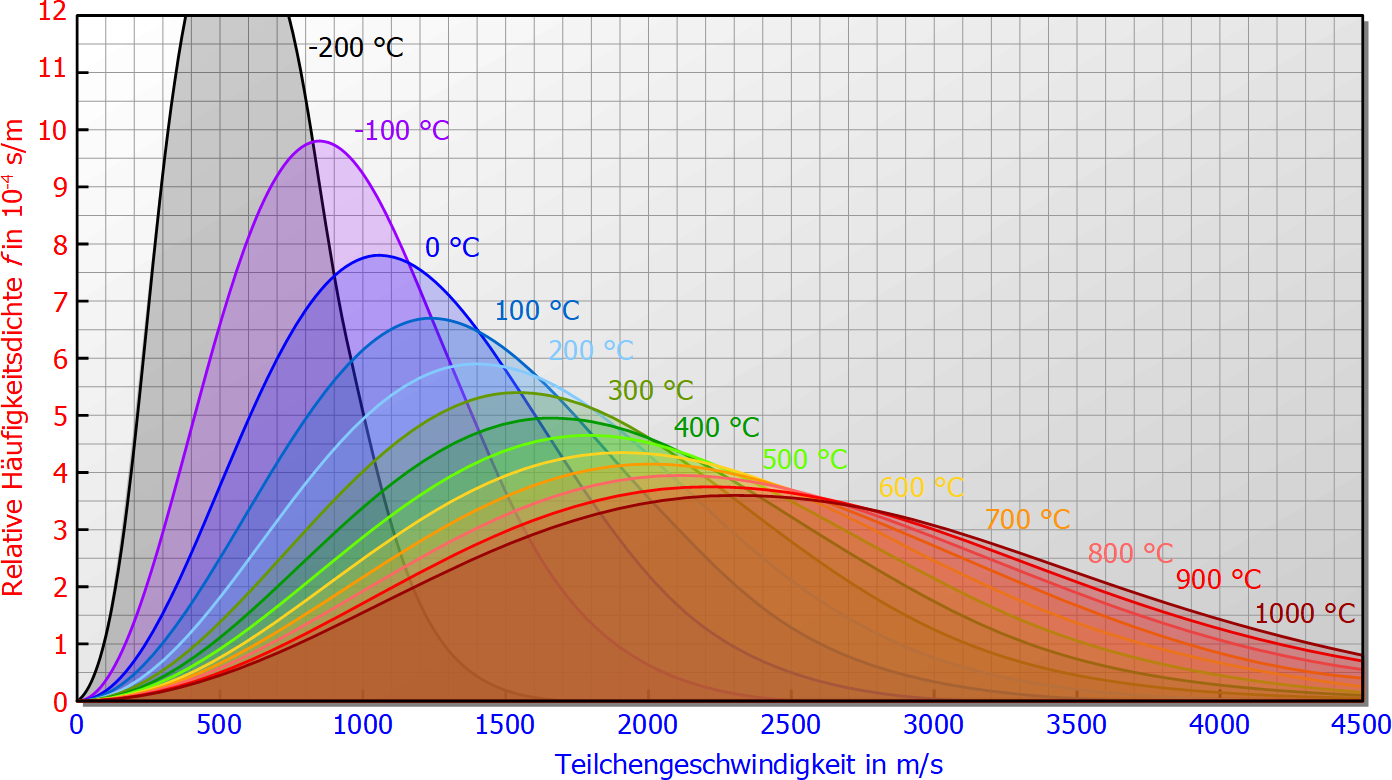
\includegraphics[width=0.75\textwidth]{img/boltzmann}
	\caption{Boltzmann-Verteilung}
\end{figure}
\FloatBarrier
%Ende

\newpage

\subsection{Allg. Beschreibung 1. HS Thermodynamik}
\begin{center}
	"`die innere Energie eines abgeschlossenen Systems bleibt konstant."'\\
	d$U=0$ bzw. $U=const.$
\end{center}

\textbf{\underline{Folgesätze, die sich daraus ergeben:}}
\begin{itemize}
	\item \textbf{Energieerhaltungssatz}:\\
	"`Energie kann weder erzeugt noch zerstört werden, sondern nur in eine andere Energieform umgewandelt werden."'
	\item Energie ist die Fähigkeit zum \textbf{Austausch von Arbeit und Wärme}
	\item innere Energie $ U $ und Enthalpie $ H $ beschreiben System als \textbf{Zustandsgrößen}
	\item In einem \textbf{Kreisprozess wird keine Energie gewonnen}, wenn bei Rückkehr auf einen beliebigen Weg vom Zustand 2 in den Ausgangszustand 1, die gleiche Summe von Wärme und Arbeit mit umgekehrten Vorzeichen ausgetauscht wird
\end{itemize}
\textbf{\underline{Arbeits- und Energietherme:}}
\begin{itemize}
	\item \textbf{Volumenarbeit} $W_V = F*s \rightarrow \text{d}W=p*A*\text{d}s=-p*\text{d}V $
	\begin{itemize}
		\item $U$ sinkt: Expansion
		\item $U$ steigt: Kompression
	\end{itemize}
	\textbf{Fall A:} Arbeit gegen $p_u,T=const.$
	\begin{flalign}
		&\text{d}W=-p*\text{d}V\\
		&\Delta W = W_2-W_1=\int_{V_1}^{V_2}-p_u\text{ d}V\\
		&\Delta W =-p_u\int_{V_1}^{V_2}\text{d}V=-p*(V_2-V_1)\\
 	\end{flalign}
 	\textbf{Fall B:} Arbeit gegen $T=const., p\neq const.$
 	\begin{flalign}
 	&\text{d}W=-p*\text{d}V\\
 	&\Delta W =\int_{V_1}^{V_2}-p\text{ d}V\\
 	&\Delta W =\int_{V_1}^{V_2}-\frac{n*R*T}{V}\text{ d}V\\
 	&\Delta W = -n*R*T* \int_{V_1}^{V_2}\frac{1}{V}\text{ d}V\\
 	&\Delta W = -n*R*T*\ln{\left(\frac{V_2}{V_1}\right)}
 	\end{flalign}
\end{itemize}

\newpage

\subsection{Totales Differential der inneren Energie U}
\begin{itemize}
	\item Abhängigkeiten von $U$ für ein gasförmiges System: $\text{ }U=f(p,T,V,n,...)$\\
	Innere Energie U (gasförmiges System) abhängig von Druck P, Volumen V, Temperatur T, Teilchenzahl n
	\item Beschreibung der Abhänigkeit von $U$ von den Größen p,T,V,... erfolgt als totales Differential\\
		\begin{flalign}
			\text{d}U &= \left(\frac{\partial U}{\partial T}\right)_{V,n}*\text{d}T+\left(\frac{\partial U}{\partial V}\right)_{T,n}*\text{d}V+\left(\frac{\partial U}{\partial n}\right)_{V,T}*\text{d}n
		\end{flalign}
		$\rightarrow$ für $n=const.$
		\begin{flalign}
		\text{d}U &= \left(\frac{\partial U}{\partial T}\right)_{V,n}*\text{d}T+\left(\frac{\partial U}{\partial V}\right)_{T,n}*\text{d}V
		\end{flalign}
		\begin{center}
			Wärmekapazität $c_V$ \hspace*{5mm} Binnendruck $\pi$\\
			bei $V=const.$ \hspace*{30mm}
		\end{center}
\end{itemize}

In jedem geschlossenem System ist jede infinitial kleine Änderung der Inneren Energie den jeweiligen Änderungen von Volumen und Temperatur proportional.\\
Proportionalitätsfaktoren sind dabei partielle Ableitungen nach den Zustandsvariablen $T,V \text{ und } n=const.$

\subsubsection{Temperaturabhängigkeit der inneren Energie $\mathbf{U}$}
\begin{flalign}
	\diff U &= \diff W +\diff Q\\
	Q_{12} &= (U_2-U_1)-W_{ges 1,2}\\
	q_{1,2} &= (u_2-u_1)-w_{ges 1,2}
\end{flalign}
Nur Volumenarbeit, vollständig reversibler Prozess\\

\begin{table}[h!]
	\centering
	\begin{tabulary}{1.15\textwidth}{C|C|C}
		System mit $p=const.$ u. $p\neq f(V)$ & System mit $p\neq const.$ & System mit konst. Volumen $\diff W_{Vol}=0$ \\  
		$q_{12}=(u_2-u_1)-p*(v_2-v_1)$& $q_{12}=(u_2-u_1)-n*R*T*\ln\left(\frac{v_2}{v_1}\right)$ & $q_{12}=(u_2-u_1)$
	\end{tabulary} 
\end{table}
\FloatBarrier

\newpage

\subsubsection{Wärmekapazität $\mathbf{c_V}$ bei konstantem Volumen}
\begin{flalign}
	\diff U =\left(\frac{\partial U}{\partial T}\right)_{V,n}*\diff T
\end{flalign}
\vspace*{-5mm}\\
\hspace*{70mm} $\hookrightarrow c_V$\\
\begin{itemize}
	\item $c_V$ gibt an wie stark sich die innere Energie des Systems mit der Temperatur $(v=const.)$|adiabat
	\item $c_V=$"'groß"': \\
	hohe Wärmekapazität, stärkere Änderung von $U$, Teilchen können "`viel"' Energie aufnehmen 
	\begin{itemize}
		\item frei beweglich
		\item  viele Teilchen
		\item Rotation, Translation, Vibration
		\item wenig Doppelbindung
	\end{itemize}
	\item Wärmekapazität ist selbst wieder eine temperaturabhängige Größe\\
	Generell gilt:
	\begin{itemize}
		\item für $T\rightarrow \SI{0}{\kelvin}$ mit $c_V \rightarrow 0$
		\item für Phasenwechsel mit $c_V\rightarrow \infty$
	\end{itemize}
\end{itemize}

\subsubsection{Volumenabhängigkeit der inneren Energie $\mathbf{U}$}
\textbf{Der Binnendruck $\mathbf{\pi}$}
\begin{flalign}
	\diff U &= \left(\frac{\partial U}{\partial T}\right)_{V,n}*\diff T+\left(\frac{\partial U}{\partial V}\right)_{T,n}*\diff V
\end{flalign}
für $n=const.$
\begin{flalign}
	\diff U &= c_v+\diff T + \pi *\diff V
\end{flalign}
\vspace*{-10mm}\\
\hspace*{85mm} $\uparrow$ Binnendruck

Der Binnendruck $\pi$ ist eine Maß für die Änderung der inneren Energie eines Stoffes, wenn sich Volumen bei $T=const.$ ändert

\begin{table}[h!]
	\centering
	\begin{tabulary}{1.15\textwidth}{C|C}
		\textbf{Ideale Gase} & \textbf{Reale Gase}\\
		\hline
		$\pi =0$ 	& $\pi \uparrow$ - Abstoßung der Teilchen\\
		& $\pi \downarrow$ - Anziehung der Teilchen\\
		keine WW der Teilchen & WW zwischen den Teilchen
	\end{tabulary} 
\end{table}
\FloatBarrier

\newpage

\subsection{Modellsystem "`Ideales Gas"' und Verhalten realer Gase}
\subsubsection{Annahmen zum idealen Gas}
\begin{itemize}
	\item Energie nur in Form kinetischer Energie\\
	$\rightarrow$ potentielle Energie wird aufgrund WW mit Atomen/Molekülen vernachlässigt
	\item Stöße zwischen Teilchen vollständig elastisch\\
	$\rightarrow$ keine E-Umwandlung durch Verformung,...
	\item kein Eigenvolumen der Teilchen
	\item Teilchen sind in zufälliger Bewegung zueinander (kontinuierlich)\\
	$\rightarrow$ Energie verteilt sich auf Energieniveaus\\
	$\rightarrow$ Verteilung der Teilchengeschwindigkeit 
	\item Größe der Teilchen vernachlässigbar, da $<<<$ mittlere, freie Weglänge \\
	("`Weg vor Stoß"')
\end{itemize}


\subsubsection{Verhalten realer Gase}

\begin{itemize}
	\item WW der Teilchen
	\item Eigenvolumen
	\item inelastische Stöße
	\item statistisch nicht mehr zufällige Bewegung
\end{itemize}

\textbf{KONSEQUENZ:}\\
Die Zustandsgrößen $p$ und $V$ zeigen in der/ihrer Berechnung Abweichungen, wenn sie nicht mit einem entsprechenden korrigierten Gasgesetz bestimmt bzw. berechnet werden.

\begin{center}
	\textbf{Übergangslösung:}
	\begin{itemize}
		\centering
		\item bei Experiment hohe Temperaturen und niedrige Drücke
		\item Nutzung des ideales gases zum Überblick
	\end{itemize}
\end{center}

\newpage

\textbf{LÖSUNGSMÖGLICHKEITEN:}
\begin{itemize}
	\item \textbf{Einsatz von Korrekturfaktoren}
	\begin{itemize}
		\item Kompressibilität $z$
		\item Fugazitäten- und Fugazitätskoeffizienten $f_{\text{i}}$ und $\Phi_{\text{i}}$
		\item Aktivität- und Aktivitätskoeffizienten $a_{\text{i}}$ und  $\gamma_{\text{i}}$\\
			$a_{\text{i}}=\gamma_{\text{i}}*c_{\text{i}}$ mit $\gamma_{\text{i}}=1,0$ als 100\% ideal
	\end{itemize}
	
	\item \textbf{Erweiterung des idealen Gasgesetzes}
	\renewcommand{\arraystretch}{1.2}
	\begin{table}[h!]
		\centering
		\begin{tabulary}{\textwidth}{C|C}
			\textit{Erweiterung durch die Einführung von Zusatzgliedern} & \textit{Einführung von Korrekturtermen in das ideale Gasgesetz} \\
			\hline
			&\\
			Reihenentwicklung & Korrekturtherme\\
			"`Virialgleichungen"'& Van-der-Waals GL, Berthelot GL, Redlich-K.-Wong GL, Peng-Robinson GL
		\end{tabulary} 
	\end{table}
	\FloatBarrier
\end{itemize}








\subsection{Zustandsgleichung und Gasgesetze}
\subsubsection{Charakterisierung der Gasphase am Beispiel von Wasser-Dampf-Gemischen}
System A = \\
Mischung aus flüssiger Phase (F,$'$) und gasförmiger Phase (Dampf D, $''$)
\begin{flalign}
	V_A &= m_D*V''+m_F*V'\\
	V_{m_A} &= \frac{V_A}{n} \quad V_A = \frac{v_A}{m_A}\\
	\chi_{\text{i}} &= \frac{n_{\text{i}}}{n_{\text{ges}}} = \frac{m_{\text{i}}}{m_{\text{ges}}}\\
	v_A &= \chi_D *v''+\chi_F*v'\\
		&= \chi_D *v''+(1-\chi_D)*v'\\
		&= \chi_D *v''+v'-\chi_D*v'\\
		&= v''+\chi_D*(v''-v')\\
	\chi_D &=\frac{v_A-v'}{v''-v'}
\end{flalign}

\begin{itemize}
	\item Eigenschaften der D-F-mischung sind abhängig von den Massen- bzw. Molenbrüchen der Phasen
	\item Jedes Zweiphasengebiet kann jeden Punkt genau durch Temperatur und Druck bestimmen \\
	$\rightarrow$ Freiheitsgrad = 1 $\rightarrow F=K-P+2$
	\item Dampf-Tafeln für verschiedene Stoffsysteme mit spezifischen Zustandsgrößen $v,h,s$
\end{itemize}

\subsubsection{Analoge Betrachtung für ander thermodynamische Größen}
\textbf{Enthalpie:}\\
\begin{flalign}
	H_A 	&= m_D * H'' +m_F*H'\\
	\chi_D 	&= \frac{h_A-h'}{h''-h'}\\
	h_A		&= \chi_D*(h''-h')+h'
\end{flalign}
\textbf{Entropie:}\\
\begin{flalign}
S_A 	&= m_D * S'' +m_F*S'\\
\chi_D 	&= \frac{s_A-s'}{s''-s'}\\
s_A		&= \chi_D*(s''-s')+s'
\end{flalign}


\subsection{Kinetische Gastheorie}

ABBILDUNG \\

\textbf{Reduzierte Masse $\mathbf{\mu}$}
\begin{flalign}
	\mu 		&= m_{Red} \quad \quad \quad \quad \quad \quad \text{(einatomig)}\\
	\mu &= m_{Red} = \frac{m_1*m_2}{m_1+m_2} \text{ (zweiatomig)}
\end{flalign}

\subsubsection{Impuls und Impulsänderung}

\begin{enumerate}
	\item 	\begin{flalign}
				\Delta p_x 	&= \mu*V_X-\mu *(-V_x)\\
							&= 2 \mu * V_x
			\end{flalign}
	\item Für zwei Treffer auf eine Wand muss ein Teilchen 2x die Strecke $l$ zurücklegen
	\begin{flalign}
				\Delta t= \frac{2*t}{V_x}
	\end{flalign}
	\item Für die ausgeübte Kraft (=Druck) an der Wand ergibt sich:
	\begin{flalign}
		F &= \frac{\Delta p_x}{\Delta t} = \frac{\mu*V_x^2}{l}\\
		p_{{\tiny Druck}} &=\frac{F}{A} = \frac{\mu*V_x^2}{l*A} = \frac{\mu*V_x^2}{V}
	\end{flalign}
	\item Berücksichtigung der Teilchenzahl $N$ (ausschließlich translatorische Freiheitsgrade x-Richtung)
	\begin{flalign}
		\bar{v}^2 	&= v_x^2+v_y^2+v_z^2\\
		p*V 		&= \frac{1}{3}*N*\mu*\bar{v}^2	 
	\end{flalign}
	Für 1 mol Teilchen ergibt sich:
	\begin{flalign}
		N 	&= n*N_A \\
		n 	&= \frac{m}{M}=\frac{\mu}{M}\\
		p*V &= n*M_{ges}*\bar{v}^2
	\end{flalign}
	\item Wenn die neu gefundene Gleichung als Zustandsgleichung für das ideale Gas gelten soll, können wir nachfolgend auch den Ausdruck $n*R*T$ mit in die Gleichung integrieren
	\begin{flalign}
		\frac{1}{3}*N*\mu*\bar{v}^2 &= n*R*T\\
		\frac{1}{3}*n*M_{ges}*\bar{v}^2 &= n*R*T\\
	\end{flalign}
	\begin{flalign}
		k_B &= \SI{1,38e-23}{\joule \per \kelvin}\\
		R 	&= \SI{8,314}{\joule\per\kelvin\per\mole}\\
		N_A &= \SI{6,02e23}{\per\mole}
	\end{flalign}
	$\rightarrow$ mit $R=k_B*N_A$ \\
	\begin{flalign}
		\bar{v} 	&= \sqrt{\frac{3*R*T}{N*\mu}}\\
					&= \sqrt{\frac{3*R*T}{M}}\\
					&= \underline{\underline{\sqrt{\frac{3*k_B*T}{\mu}}}}
	\end{flalign}
	\item \textbf{Schlussfolgerung:}
	\begin{flalign}
		\bar{v}^2 \sim T \text{ und } \bar{v}^2 \sim \frac{1}{\mu} \text{ bzw. } \frac{1}{M}\\
		p*V = N *k_B*T
	\end{flalign}
\end{enumerate}

\subsubsection{Boltzmann Verteilung}

ABBILDUNG\\

=Beschreibt Einfluss von $T$ auf Geschwindigkeitsverteilung der Teilen, sowie der Molmasse $M$ bzw. reduzierten Masse $\mu$

\subsubsection{Mittlere quadratische Geschwindigkeit $\mathbf{\bar{v}}$}
\begin{flalign}
	\bar{v}^2 	&= \frac{3*R*T}{M}\\
	\bar{v}		&= \sqrt{\frac{3*R*T}{M}}
\end{flalign}
\underline{Bsp.:} $CO_2$ mit $\bar{v}= \SI{411}{\meter \per \second}$

\subsubsection{Mittlere Geschwindigkeit $\mathbf{c}$}
\begin{itemize}
	\item aus Maxwell Gleichung
	\item jede Geschwindigkeit wird multipliziert mit Teilchenzahl, die diese Geschwindigkeit besitzen
	\item Aufsummation aller Produkte und Mittelung
\end{itemize}
\begin{flalign}
	c 		&= \int_{0}^{\infty} s*f(s)*\diff s\\
	f(s) 	&= 4*\pi*\left(\frac{M}{2*\pi*T*R}\right)^{\frac{3}{2}}*s^2*e^{-\frac{M*s^2}{2*R*T}}\\
	c		&= 4*\pi*\left(\frac{M}{2*\pi*T*R}\right)^{\frac{2}{3}}*\frac{1}{2}*\left(\frac{2*R*T}{M}\right)^2\\
	c		&= \underline{\underline{\left(\frac{8*R*T}{\pi*M}\right)^{\frac{1}{2}}}}
\end{flalign}
